\chapter[The discrete Radon transform]{Calculating the discrete Radon transform}
\label{ch:RadonCalc}

In this appendix, we demonstrate how the Radon transform is calculated for a discretised velocity distribution, as described in Chapter~\ref{ch:directional}. We first consider calculating the azimuthally averaged Radon transform of a general velocity distribution $f(\textbf{v})$:

\begin{align}
\label{eq:RadonCalc:fullRadon}
\hat{f}(\vmin, \cos\theta) &= \int_0^{2\pi} \hat{f}(\vmin, \cos\theta, \phi) \, \mathrm{d}\phi \notag\\
&= \int_0^{2\pi}\left( \int_{\mathbb{R}^3} f(\mathbf{v}) \delta\left(\mathbf{v}\cdot\hat{\mathbf{q}} - \vmin \right)\, \mathrm{d}^3\mathbf{v} \right) \mathrm{d}\phi \\
&= \int_{\phi = 0}^{2\pi} \int_{v = 0}^{\infty} \oint \frac{1}{v} f(\textbf{v}) \delta\left(v_\textrm{min}/v - \hat{\textbf{v}}\cdot\hat{\textbf{q}}\right) \, \mathrm{d}\Omega_v \mathrm{d}v \mathrm{d}\phi \notag\,.
\end{align}
We recall that primed angles $(\theta',\phi')$ are associated with the direction of $\textbf{v}$, while unprimed angles $(\theta, \phi)$ are associated with the direction of $\hat{\textbf{q}}$. Thus, the $\phi$ integral in Eq.~\ref{eq:RadonCalc:fullRadon} applies only to the $\delta$-function. Expanding the dot product into angular coordinates, we write the $\phi$ integral as

\begin{align}
I(\vmin, \cos\theta, \mathbf{v}) &= \int_{0}^{2\pi} \delta\left(\sin\theta\sin\theta' \cos(\phi-\phi') + \cos\theta\cos\theta' - \vmin/v\right) \label{eq:defI} \, \mathrm{d}\phi \notag\\
&\equiv \int_{0}^{2\pi} \delta\left(g(\phi)\right) \, \mathrm{d}\phi\,.
\end{align}
We then rewrite the delta function as a function of $\phi$:
\begin{equation}
\label{eq:RadonCalc:deltadecomp}
\delta\left(g(\phi)\right) = \sum_{i} \frac{\delta(\phi - \phi_i)}{|g'(\phi_i)|}\,.
\end{equation}
Here, we sum over those values of $\phi_i$ satisfying $g(\phi_i) = 0$,

\begin{align}
\label{eq:RadonCalc:gamma}
g(\phi_i) &= 0 \notag\\
\Rightarrow \cos(\phi_i - \phi') &= \frac{\beta - \cos\theta\cos\theta'}{\sin\theta \sin\theta'} \equiv \gamma\,,
\end{align}
where we have also defined $\beta = \vmin/v$. The solutions for $\phi \in [0,2\pi]$ are:
\begin{align}
\phi_1 &= \phi' + \acos\gamma, & \textrm{ for } &  \phi' \in \left[0, 2\pi - \acos\gamma\right] \notag\\
\phi_2 &= \phi' + 2\pi - \acos\gamma, & \textrm{ for } & \phi' \in \left[0, \acos\gamma\right] \notag\\
\phi_3 &= \phi' + \acos\gamma -2\pi, & \textrm{ for } & \phi' \in \left[2\pi - \acos\gamma, 2\pi\right] \notag\\
\phi_4 &= \phi' -\acos\gamma, & \textrm{ for } & \phi' \in \left[\acos\gamma, 2\pi\right] \,.
\end{align}
We note that these solutions exist only for $\beta \in \left[0,1\right]$ (or equivalently $v > \vmin$) and for $\gamma \in [-1,1]$, otherwise Eq.~\ref{eq:RadonCalc:gamma} cannot be satisfied. If these constraints are satisfied, there exist exactly 2 solutions for a given value of $\phi'$ and therefore 2 $\delta$-functions in Eq.~\ref{eq:RadonCalc:deltadecomp}.

For the derivative of $g(\phi)$ we obtain
\begin{align}
g'(\phi) = -\sin\theta\sin\theta'\sin(\phi-\phi')\,.
\end{align}
Substituting the values of $\phi_{1,2,3,4}$, we see that
\begin{align}
|g'(\phi_{1,2,3,4})| = \sqrt{\left(\sin\theta\sin\theta'\right)^2 - \left(\beta - \cos\theta\cos\theta'\right)^2}\,.
\end{align}
Each of the two $\delta$-functions therefore contributes the same amount to the integral, regardless of the value of $\phi'$. Performing the integral, we obtain

\begin{equation}
I(\vmin, \cos\theta, \mathbf{v}) = \frac{2 C(\gamma)}{\sqrt{\left(\sin\theta\sin\theta'\right)^2 - \left(\beta - \cos\theta\cos\theta'\right)^2}}\Theta(v - \vmin)\,,
\end{equation}
where $C(\gamma) = 1$ for $\gamma \in [-1,1]$ and vanishes otherwise.

We therefore obtain

\begin{equation}
\hat{f}(\vmin, \cos\theta) = \int_{-1}^{1} \int_{\vmin}^{\infty}  f(v, \cos\theta') I(\vmin, \cos\theta, v, \cos\theta')\, v \mathrm{d}v\, \mathrm{d}\cos\theta'\,,
\end{equation}
where we have performed the $\phi'$ integral over the velocity distribution,
\begin{equation}
f(v, \cos\theta') = \int_{0}^{2\pi} f(v, \cos\theta', \phi') \, \mathrm{d}\phi'\,,
\end{equation}
because $I(\vmin, \cos\theta, \mathbf{v})$ does not depend on $\phi'$. In order to make further progress, we need an explicit form for $f(v, \cos\theta')$. We now consider the discretised velocity distributions discussed in Chapter~\ref{ch:directional}.


\section{$N=2$ discretisation}

For the $N=2$ case, we are considering a forward-backward asymmetry in the velocity distribution:

\begin{equation}
\label{eq:RadonCalc:N2}
f(\mathbf{v}) =
\begin{cases}
f^1(v) & \textrm{for } \theta' \in [0, \pi/2] \\
f^2(v) & \textrm{for } \theta' \in [\pi/2, \pi]\,.
\end{cases}
\end{equation}

From these, we wish to obtain the integrated Radon transforms for the forward and backward directions. Specifically:

\begin{align}
\hat{f}^1 &= \int_{0}^1 \hat{f}(v_q,\cos\theta) \, \mathrm{d}\cos\theta \\
\hat{f}^2 &= \int_{-1}^0 \hat{f}(v_q, \cos\theta) \, \mathrm{d}\cos\theta \,.
\end{align}
We will focus on the first of these, $\hat{f}^1$, as the other can be obtained simply by exchanging which directions are forward and backward (that is, by interchanging $f^1$ and $f^2$). From now on, we will therefore be working under the assumption that $\cos\theta \in [0,1]$.

We start with the $\cos\theta'$ integral:

\begin{align}
\label{eq:RadonCalc:J}
J \equiv &\int_{-1}^{1} f(v, \cos\theta')I(\vmin, \cos\theta, v, \cos\theta') \, \mathrm{d}\cos\theta' \nonumber\\
&\qquad = 2\pi\int_0^1 f^1(v) I(\cos\theta') \, \mathrm{d}\cos\theta' + 2\pi\int_{-1}^0 f^2(v) I(\cos\theta') \, \mathrm{d}\cos\theta'\,.
\end{align}
The factor $C(\gamma)$ in the expression for $I$ requires that $|\gamma| < 1$. We can show that this is equivalent to requiring that $\cos\theta' \in [x_-, x_+]$, where

\begin{equation}
x_{\pm} = \beta\cos\theta \pm \sqrt{1-\beta^2}\sin\theta\,.
\end{equation}
We show $x_{\pm}$ as a function of $\cos\theta$ in Fig.~\ref{fig:RadonCalc:IntegLimits}. Focusing on $\cos\theta \in [0,1]$, we note that there are two distinct regimes. For $\cos\theta \in [0, \sqrt{1-\beta^2}]$, $x_+$ is positive, while $x_-$ is negative. For $\cos\theta \in [\sqrt{1-\beta^2},1]$, however, both $x_+$ and $x_-$ are positive. We therefore need to treat these two cases separately. Equation~\ref{eq:RadonCalc:J} then becomes

\begin{align}
J &= \int_{x_-}^{0} \frac{4\pi f^2(v) \, \mathrm{d}\cos\theta'}{\sqrt{\left(\sin\theta\sin\theta'\right)^2 - \left(\beta - \cos\theta\cos\theta'\right)^2}}  \\
& +\int_{0}^{x_+} \frac{4\pi f^1(v) \, \mathrm{d}\cos\theta'}{\sqrt{\left(\sin\theta\sin\theta'\right)^2 - \left(\beta - \cos\theta\cos\theta'\right)^2}}, & \textrm{ for } \cos\theta \in [0,\sqrt{1-\beta^2}] \nonumber\\
J &= \int_{x_-}^{x_+} \frac{4\pi f^1(v) \, \mathrm{d}\cos\theta'}{\sqrt{\left(\sin\theta\sin\theta'\right)^2 - \left(\beta - \cos\theta\cos\theta'\right)^2}}, & \textrm{ for } \cos\theta \in [\sqrt{1-\beta^2},1]\,.
\end{align}

\begin{figure}[tbh!]
  \centering
  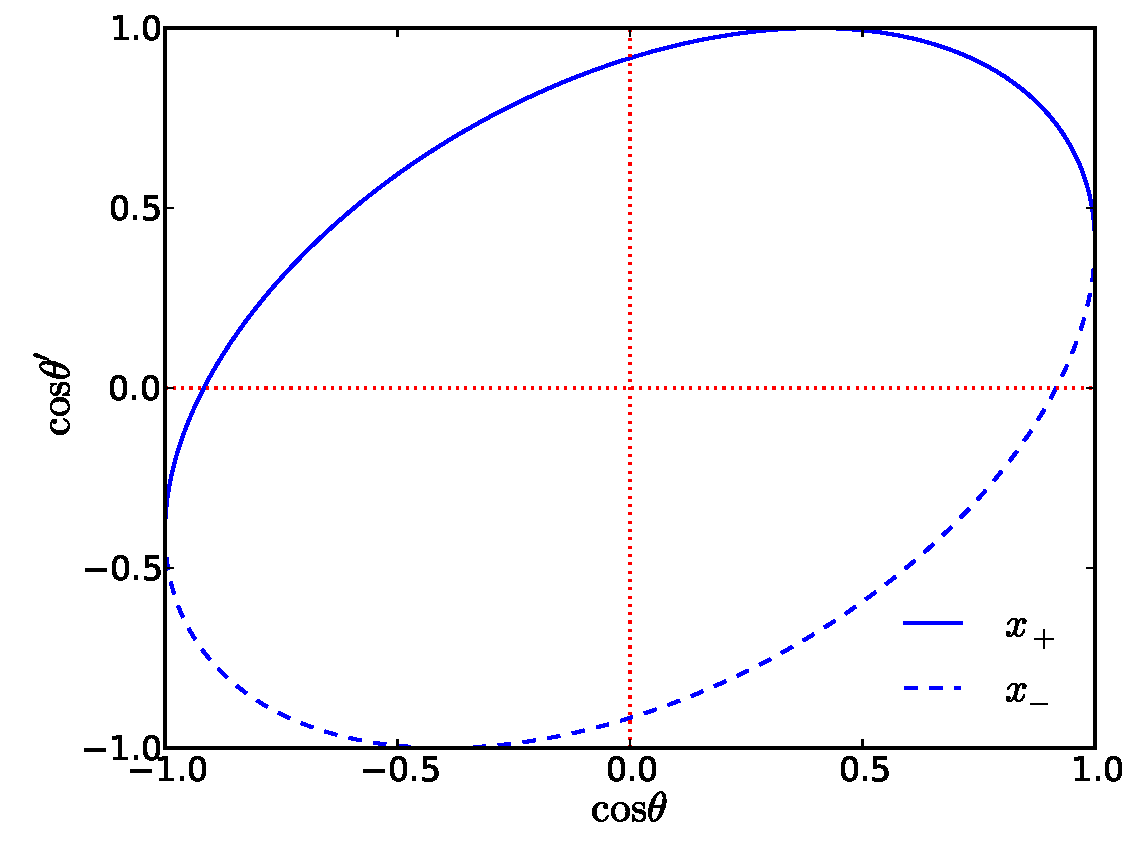
\includegraphics[width=0.75\textwidth]{Directional/Integlimits.pdf}
\caption[Integration limits in the calculation of the Radon transform]{Integration limits for Eq.~\ref{eq:RadonCalc:J} as a function of $\cos\theta$, for a fixed value of $\beta$. The value $\cos\theta' = 0$ is denoted with a horizontal dashed line, while $\cos\theta = 0$ is shown with a vertical dashed line.}
  \label{fig:RadonCalc:IntegLimits}
\end{figure}

We note that
\begin{equation}
\int_{x_1}^{x_2} \frac{\, \mathrm{d}\cos\theta'}{\sqrt{\left(\sin\theta\sin\theta'\right)^2 - \left(\beta - \cos\theta\cos\theta'\right)^2}} = \left[\asin\left(\frac{x-\beta\cos\theta}{\sqrt{1-\beta^2}\sin\theta}\right)\right]_{x_1}^{x_2}\,,
\end{equation}
so that $J$ takes the form:

\begin{align}
J &= 4\pi f^1(v)\left(\frac{\pi}{2} + \asin\left\{\frac{\beta\cos\theta}{\sqrt{1-\beta^2}\sin\theta}\right\}\right) \nonumber \\
& + 4\pi f^2(v)\left(\frac{\pi}{2} - \asin\left\{\frac{\beta\cos\theta}{\sqrt{1-\beta^2}\sin\theta}\right\}\right) & \textrm{ for } \cos\theta \in [0,\sqrt{1-\beta^2}] \nonumber \\
J &= 4\pi^2 f^1(v), & \textrm{ for } \cos\theta \in [\sqrt{1-\beta^2},1]\,.
\end{align}

We finally perform the $\cos\theta$ integral:

\begin{equation}
\hat{f}^1 = \int_{0}^{1} \int_{\vmin}^{\infty}  J \, v \mathrm{d}v \mathrm{d}\cos\theta\,.
\end{equation}
Noting that
\begin{align}
\label{eq:RadonCalc:K0}
&\int_{x_1}^{x_2} \asin\left(\frac{\beta\cos\theta}{\sqrt{1-\beta^2}\sin\theta}\right) \,\mathrm{d}\cos\theta \notag\\
& =\left[ x \asin\left(\frac{\beta x}{\sqrt{1-\beta^2}\sqrt{1-x^2}}\right) + \atan\left(\frac{1}{\beta}\sqrt{1-\beta^2 -x^2}\right)\right]_{x_1}^{x_2}\,,
\end{align}
we obtain

\begin{align}
\label{eq:RadonCalc:N2result}
\hat{f}^1 &= 4\pi\int_{\vmin}^{\infty} v \left( \pi f^1(v) + \atan\left(\frac{\sqrt{1-\beta^2}}{\beta}\right)\left[f^2(v) - f^1(v)\right] \right) \, \mathrm{d}v \\
\hat{f}^2 &= 4\pi\int_{\vmin}^{\infty} v \left( \pi f^2(v) + \atan\left(\frac{\sqrt{1-\beta^2}}{\beta}\right)\left[f^1(v) - f^2(v)\right] \right) \, \mathrm{d}v\,,
\end{align}
where $\hat{f}^2$ is obtained by exchanging $f^1(v)$ and $f^2(v)$.

\section{$N=3$ discretisation}

The calculation of the forward, backward and transverse Radon transforms for $N=3$ discretisation proceeds as in the $N=2$ case. However, we must divide the integration regions of Fig.~\ref{fig:RadonCalc:IntegLimits} into 3 regions rather than into 2 regions. In addition, in the $N=3$ case, $x_\pm$ lie in different ranges of $\cos\theta'$ depending on the value of $\beta$. Thus, we must also take care to divide the range of $v$ into distinct regions depending on which angular bin $x_\pm$ fall into. We will not present the result of the calculation here, as its form is not particularly instructive. However, we will note that we require a generalised version of Eq.~\ref{eq:RadonCalc:K0} in order to perform the calculation:

\begin{align}
&\int \asin\left(\frac{y -\beta\cos\theta}{\sqrt{1-\beta^2}\sin\theta}\right) \,\mathrm{d}\cos\theta \notag\\
&= x \asin\left(\frac{y-\beta x}{\sqrt{1-x^2}\sqrt{1-\beta^2}}\right) \notag\\
&\, + y \atan\left(\frac{x-y\beta}{\sqrt{t}}\right) \notag\\
&\, + \frac{1}{2} \atan\left(\frac{1 - y^2 - \beta^2 - x + y\beta(1+x)}{(y-\beta) \sqrt{t}}\right) \notag\\
&\, - \frac{1}{2} \atan\left(\frac{1 - y^2 - \beta^2 + x - y\beta(1-x)}{(y+\beta) \sqrt{t}}\right) + C \notag\\
&\equiv K(x;y) + C\,,
\end{align}
where it is understood that $K(x;y)$ is a function of $\beta$ and where
\begin{equation}
t = (1-x^2)(1-\beta^2) - (y - \beta x)^2\,.
\end{equation}
The full results are then in the form of 1-dimensional integrals over these sums of elementary functions. The fact that an analytic integral can be performed for any value of $y$ means that we can calculate the Radon transform for any values of the $\theta'$ bin edges and therefore extend the method up to any value of $N$.

\begin{comment}
The result for the $N=3$ discretisation is then

\note{Check overall factors...}


\begin{align}
&\hat{f}^1(\vmin) = \int_{1/2}^{1} \hat{f}(\vmin,\cos\theta) \, \mathrm{d}\cos\theta \notag \\
&= \int_{\vmin}^{2\vmin} v\left\{\pi f^1(v) + (f^2(v) - f^1(v))\left(\frac{\pi}{2}(A_1 - \frac{1}{2}) + K(A_1;\half) - K(\half;\half)\right)\right\} \, \mathrm{d}v \notag\\
%&+ \int_{2\vmin}^{\infty} v\left\{
\end{align}
\end{comment}

